\documentclass[11pt,a4paper]{article}

\usepackage[utf8]{inputenc}
\usepackage{fullpage}
\usepackage{authblk}
\usepackage{graphicx}
\usepackage{caption}
\usepackage{subcaption}
\usepackage{amsmath}
\usepackage{amssymb}
\usepackage{bbm}
\usepackage{euscript}
\usepackage{graphicx}
\usepackage{subcaption}
\usepackage{lmodern}
\usepackage{textcomp}
\usepackage{titlesec}
\usepackage{float}
\usepackage{amsfonts}
\usepackage{bm}
\usepackage{stmaryrd}
\usepackage{bbm}


\usepackage{color}
\definecolor{myorange}{rgb}{0.9568,0.4941,0.1961}
%\definecolor{myred}{rgb}{0.9098,0.1294,0.2078}
\definecolor{myblue}{rgb}{0.0352,0.4981,0.6509}
%\definecolor{mygreen}{rgb}{0.2235,0.6353,0.2588}
\definecolor{lightgray}{rgb}{0.8,0.8,0.8}
%\definecolor{myhyperblue}{rgb}{0.1607,0.3922,0.9}
\definecolor{mygrey}{rgb}{0.3,0.3,0.3}

% colorblind scheme
\definecolor{myred}{rgb}{0.8509,0.3725,0.0549}
\definecolor{myhyperblue}{rgb}{0.1725, 0.4980, 0.7215}
\definecolor{mygreen}{rgb}{0.4980, 0.8039, 0.7333}

\newcommand{\unknown}[1]{\bm{{\color{myred}{#1}}}}
\newcommand{\param}[1]{\bm{{\color{myhyperblue}{#1}}}}
\newcommand{\data}[1]{\bm{{\color{mygreen}{#1}}}}
\newcommand{\keyword}[1]{[\texttt{\textbf{#1}}]\!\,}

\title{Functional scope \texttt{wave1D v1}: piezoelastic models}

\author[1]{Florian Le Bourdais, Alexandre Imperiale}

\begin{document}

% \bibliographystyle{apalike}

\maketitle

\section{Continuous models}
\subsection{Strong formulations}

\begin{center}
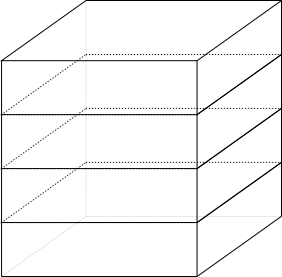
\includegraphics[scale=0.9]{figures/1dstack.png} 
\end{center}

Let $\Omega_S$ be the solid domain. Let $\Omega_P$ be the piezoelectric domain, under the assumption that  $\Omega_P \subset  \Omega_S$. The piezoelectric domain is defined by its upper point (by convention, the cathode location), $x_c$ and its lower point (by convention, the anode location), $x_a$.
\begin{equation*}
\keyword{PiezoElastic}~
\left\lbrace
\begin{aligned}
& \param{\rho}\partial^2_{tt} \unknown{u} - \partial_x\big( \param{E} \partial_x \unknown{u} \big) - \partial_x\big( \param{d} \partial_x \unknown{\varphi} \big) =  \data{f},\quad \text{in }\Omega_S,\\
& \partial_x\big( \param{\varepsilon} \partial_x \unknown{\varphi} \big) - \partial_x\big( \param{d} \partial_x \unknown{u} \big) =  0,\quad \text{in }\Omega_P,\\
& \unknown{u}(\cdot, 0) = \data{u_0},\quad \partial_t\unknown{u}(\cdot, 0) = \data{u_1},\quad \text{in }\Omega,
\end{aligned}
\right.
\end{equation*}
in the above, where $\data{u_0}(x)$ and $\data{u_1}(x)$ are input mechanical initial conditions, $\param{\rho}$ is the mass density, $\param{E}$ is the Young modulus, $\param{d}$ is the piezoelectric coupling factor and $\param{\varepsilon}$ is the electric permittivity.

\subsubsection{Electric boundary conditions}
\begin{center}
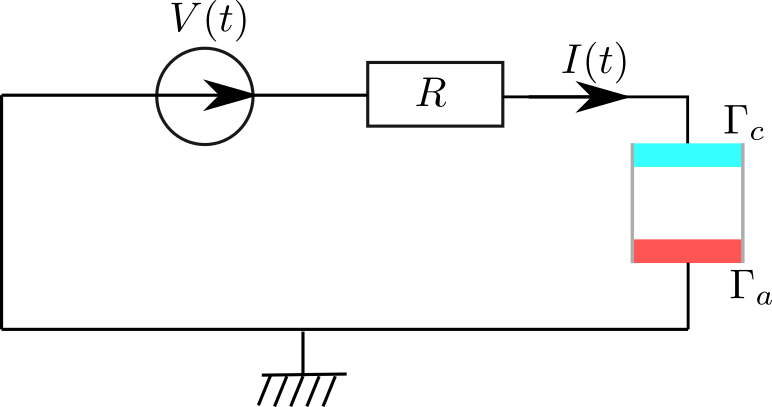
\includegraphics[scale=1]{figures/electric_circuit.png} 
\end{center}

For the above circuit, we can write the following equation on voltage:
\begin{equation*}
\begin{aligned}
\unknown{\varphi}(x_c, t) - \unknown{\varphi}(x_a, t) = \data{V}(t) + \param{R} \, \unknown{I}(t).
\end{aligned}
\end{equation*}
Since the anode is connected to the ground potential, the anode potential value $\unknown{\varphi}(x_a, \cdot)$ is 0 at all times. Additionnaly, we can write the charge $\unknown{Q}(t)$ on the cathode as a function of the potential and the displacement
\begin{equation*}
\begin{aligned}
\unknown{Q}(t) = \Big\{ \param{\varepsilon} \partial_x \unknown{\varphi}(x_c, t) - \param{d} \partial_x \unknown{u}(x_c, t) \Big\} n_P(x_c),
\end{aligned}
\end{equation*}
where $n_P$ is the normal vector to $\Omega_P$, being equal to $-1$ when at $x_c$ and $1$ when at $x_a$. In our case, this normal vector will be equal to $-1$ due to the conventions chosen. Since the current $\unknown{I}(t)$ is the time-derivative of $\unknown{Q}(t)$, we can write the following boundary conditions
\begin{equation*}
\left\lbrace
\begin{aligned}
&\unknown{\varphi}(x_a, t) = 0, \\
&\unknown{\varphi}(x_c, t) = \data{V}(t) + \param{R} \dfrac{\mathrm{d}}{\mathrm{d}t}\unknown{Q}(t).
\end{aligned}
\right.
\end{equation*}

\subsubsection{Mechanical boundary conditions}

We choose \keyword{Neumann} boundary conditions to model the solid domain $\Omega_S$
\begin{equation*}
\forall s \in\{0, L\}, \quad \left( \param{E} \partial_x \unknown{u} +  \param{d} \partial_x \unknown{\varphi} \right) n_S(s) = 0 
\end{equation*}
Here $n_S$ is the normal vector to $\Omega_S$, being equal to $-1$ when $s = 0$ and $1$ when $s=L$.

\subsubsection{Initial condition for the charge}

We choose the following initial condition for the charge of the cathode
\begin{equation*}
\unknown{Q}(0) = 0.
\end{equation*}

\subsection{Weak formulation}

\end{document}
